\vspace{.1in}
\section{Windowing} \label{sec:window}

Server programs present two challenges for \tern.  First, they 
are more exposed to
timing nondeterminism than batch programs because their inputs
(client requests) arrive nondeterministically.  Second, they often run
continuously, making their schedules too specific to reuse.

%% \begin{figure}[t]
%% \begin{center}
%% 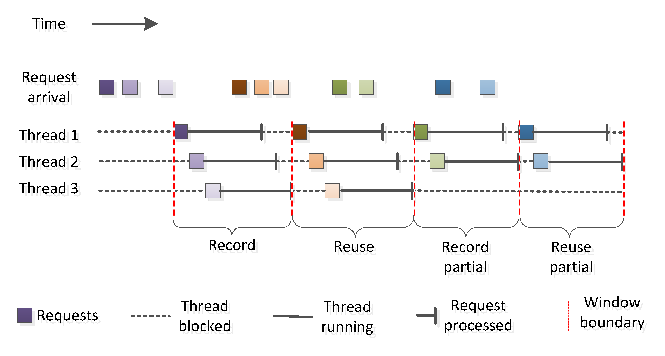
\includegraphics[width=0.47\textwidth]{figures/window-idea.eps}
%% \end{center}
%% \caption{\emph{Windowing idea.}}
%% \label{fig:window-idea}
%% \end{figure}

\tern addresses these challenges using a simple idea called
\emph{windowing}.  Our insight is that server programs tend to return to the
same quiescent states.  Thus, instead of processing requests as they
arrive, \tern breaks a continuous request stream down to windows of
requests.  Within each window, it admits requests only at fixed points in
the current schedule.  If no requests arrive at an admission point for a
predefined timeout, \tern simply proceeds with the partial window.  While a
window is running, \tern buffers newly arrived requests so that they do not
interfere with the running window.  With this approach, \tern can memoize
and reuse schedules across (possibly partial) windows.
%% Figure~\ref{fig:window-idea} illustrates this idea applied to a window
%% with four threads.  (Window size is configurable and defaults to the
%% number of CPUs.)  
The cost of windowing is that it may reduce concurrency
and degrade server throughput and speed.  However, our experiments show
that this cost is reasonable and justified by the gain in determinism
and stability.

To buffer requests, \tern needs to know when a server receives a request
and when it is done processing the request.  Inferring these task
boundaries based on thread creation and exit is unreliable because server
programs frequently use thread pools.  Thus, \tern currently lets
developers annotate these boundaries using \v{begin\_task()} and
\v{end\_task()}.  Manually locating task boundaries is often easy: a
request tends to begin after an \v{accept()} of a client connection and ends
after the server sends out a reply.

\para{Exposing hidden states.}  The assumption of windowing is that a
server program returns to the same state when it quiesces.  However, in
practice, server states evolve over time.  For instance, when Apache first
serves a page, it may load the page from disk and cache it in memory.
When this page is requested again, Apache can serve it directly from its
cache.

These state changes may affect schedules.  In the example above, Apache
will perform different synchronizations for the two runs.  Thus, for
\tern to accurately select a schedule to reuse, it must know the hidden
states that affect schedules.  Currently \tern lets developers annotate
such hidden states using \v{symbolic()}.  Doing so is often
straightforward.  For instance, we inserted a \v{symbolic()} call to mark
the return of Apache's \v{cache\_find()} as symbolic.

Exposing hidden states may not always be easy.  We thus created a
technique to tolerate missed \v{symbolic()} annotations.  The basic idea
is to store backup schedules under the same set of input constraints to
tolerate annotation inaccuracy.  For instance, suppose a \v{symbolic()}
had not been missed, \tern would have memoized two different
constraint-schedule tuples $\langle C_1, S_1 \rangle$ and $\langle C_2,
S_2 \rangle$.  However, because of the missed annotation, \tern missed the
corresponding constraints, wrongly collapsing $C_1$ and $C_2$ into the
same set $C$.  Now the two original tuples become $\langle C, S_1 \rangle$
and $\langle C, S_2 \rangle$, which appear redundant.  Instead of
discarding one of these seemingly redundant schedules, \tern will store both
schedules with the same set of constraints.  To select between these
schedules, \tern can select the one with higher reuse rate, which likely
matches the hidden state of the program.

%% For instance, Apache may store a requested page in memory, so that the
%% next request of the same page need not go to disk.  Such hidden states
%% affect schedules and should be exposed to \tern to increase schedule reuse
%% rates.

%% Currently \tern lets developers annotate such hidden states using
%% \v{symbolic()}.  Doing so is often straightforward.  For instance, we
%% inserted only one \v{symbolic()} to expose the return of Apache's
%% \v{cache\_find()} function.

%% Moreover, \tern has a mechanism to tolerate missed \v{symbolic()}
%% annotations.  The basic idea is to store backup schedules under the same
%% set of input constraints to tolerate annotation inaccuracy.  Specifically,
%% suppose a \v{symbolic()} had not been missed, \tern would have memoized
%% two different constraint-schedule tuples $\langle C_1, S_1 \rangle$ and
%% $\langle C_2, S_2 \rangle$.  However, because of the missed annotation,
%% \tern missed the corresponding constraints, wrongly collapsing $C_1$ and
%% $C_2$ into the same set $C$.  Now the two tuples become $\langle C, S_1
%% \rangle$ and $\langle C, S_2 \rangle$.  Instead of discarding one of the
%% seemly redundant schedules, \tern can store both $S_1$ and $S_2$ with $C$
%% and sort them based on reuse rates.  When looking up a schedule for an
%% input matching $C$, \tern always selects the one with the highest reuse
%% rate, which likely matches the hidden state of the program.

%% Server programs complicates
%% constraint tracking and checking as well.  During the memoization run of a
%% window, the data marked as symbolic (by \v{symbolic()} calls) may flow
%% into the server's internal state.  If the server runs for a long time,
%% this symbolic data may be examined in many branch statements, generating
%% an explosion of constraints.  Moreover, this approach mixes constraints
%% from many windows of requests together, making it difficult to check
%% constraints based only on the current window of requests.  For instance,
%% consider the Apache web server.  The currently requested page may or may
%% not be in the cache, depending on the history of requests.  Thus, to
%% determine the right schedule for the current request, we may have to
%% examine the entire history of requests.

%% To address this problem, \tern concretizes symbolic data.  Specifically,
%% After memoizing schedules for a window, \tern marks all symbolic data in
%% the current window as no longer symbolic.  It also discards symbolic
%% constraints of the current window.  This way, the symbolic data and
%% constraints do not flow into the next window.  If a later request does
%% depend on a previous request, developers can resurrect the lost
%% constraints on demand by calling \v{symbolic()} at program points where
%% the program's internal state is observed.  Locating these program points
%% tend to be easy.  For instance, we insert only one such \v{symbolic()}
%% call for Apache by marking the return of \v{cache\_find()} symbolic.

%% Moreover, \tern has a mechanism to tolerate missed \v{symbolic()}
%% annotations.  The basic idea is to store backup schedules under a set of
%% input constraints to tolerate the inaccuracy in annotations.
%% Specifically, suppose if a \v{symbolic()} had not been missed, \tern would
%% have memoized two different constraint-schedule tuples $\langle C_1, S_1
%% \rangle$ and $\langle C_2, S_2 \rangle$.  But because of the missed
%% annotation, \tern could not collect the constraints rooted from this
%% annotation, and $C_1$ and $C_2$ wrongly collapse into the same set $C$.
%% Instead of discarding one of the seemly redundant schedules, \tern can
%% store both $S_1$ and $S_2$ with $C$ and sort them based on reuse rates.
%% When looking up a schedule for an input satisfying $I$, \tern always
%% selects the schedule with the highest reuse rate, which likely matches the
%% internal state of a program.



%% %% Server programs creates two problems for \tern.  First, they run
%% %% nondeterministically because client requests nondeterministically arrive.
%% %% Second, they may run continuously, making their schedules effectively
%% %% infinite and difficult to reuse.  The second problem is made worse by
%% %% thread pools because a thread in a pool gets reused to processes many
%% %% independent user requests.  In this section, we describe how
%% %% \tern mitigates these problems.  Specifically we describe the windowing
%% %% idea (\S~\ref{sec:window-idea}), how \tern tracks and checks constraints
%% %% for windows (\S\ref{sec:window-check}), and the replacement policy of the
%% %% schedule cache (\S\ref{sec:cache-replace}).

%% %% \subsection{The Idea} \label{sec:window-idea}

%% %% \begin{figure}[t]
%% %% \begin{center}
%% %% 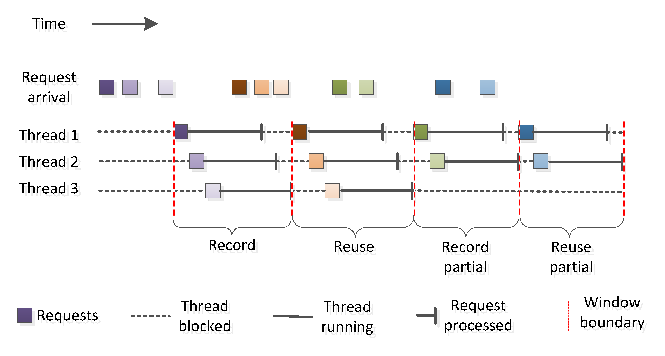
\includegraphics[width=0.47\textwidth]{figures/window-idea.eps}
%% %% \end{center}
%% %% \caption{\emph{Windowing idea.}}
%% %% \label{fig:window-idea}
%% %% \end{figure}

%% %% \tern addresses these problems using a simple idea called \emph{windowing}.
%% %% Our observation is that server programs tend to go back to the same
%% %% quiescence states once they are done processing a batch of requests.
%% %% Based on this observation, \tern breaks continuous request streams into
%% %% windows and let the server program quiesces between two windows.  \tern can
%% %% then memoize a schedule and its constraints for one window and reuse the
%% %% schedule for later windows.  Windowing also reduces input
%% %% timing nondeterminism because requests are buffered instead of immediately
%% %% processed, much like how real-time programs (\eg, mplayer) use buffers to
%% %% avoid jitter.  The downside is the loss of some concurrency, degrading
%% %% throughput and speed.  Our experiments show that the overhead of windowing
%% %% is reasonable, justified by the gain in determinism and stability.

%% %% % Windowing works for the same reason 

%% %% Figure~\ref{fig:window-idea} depicts the windowing idea using a window of
%% %% size four (\ie, \tern allows the server program to process four requests
%% %% concurrently).  As requests arrive, \tern does not process them
%% %% immediately.  When a window is full, \tern runs the server threads to
%% %% process the full window of requests.  During the run of the window,
%% %% \tern memoizes or reuses schedules as how it would for batch programs.
%% %% Moreover, \tern blocks newly arrived requests even if some server threads
%% %% are idle.  Once the window of requests are processed and the server
%% %% quiesces, \tern waits for a new window of requests.  Under light load, a
%% %% window may never become full.  \tern detects this case using a \emph{window
%% %%   timeout} (0.1 ms by default) and runs the server program on a partial
%% %% window.  It again memoizes schedules for the partial window, and blocks
%% %% new requests while the window is running.

%% %% Counter-intuitively, the higher the load, the less overhead windowing is
%% %% because under high load, windows quickly become full, avoiding the
%% %% window-detection timeout and keeping the server threads busy all the time.
%% %% Under light load, \tern has higher overhead but because the load is light
%% %% anyway, this overhead does not matter much.


%% %% must know start and end of requests.  cannot simply use thread creation and
%% %% exits because thread pools.  Thus, 

%% %% Currently \tern lets developers annotate the beginning and end of
%% %% request processing using \v{begin\_task()} and \v{end\_task()}.  Doing
%% %% so is typically easy: place \v{begin\_task(}) after an \v{accept()} of
%% %% client connection and \v{end\_task()} sends back the reply.  Developers
%% %% can also configure the window size by setting a \tern option (default to
%% %% the number of CPUs).

%% %% \subsection{Constraint Tracking and Checking} \label{sec:window-check}

%% %% Server programs complicates constraint tracking and checking as well.  The
%% %% data marked by \v{symbolic()} may flow into a server program's internal
%% %% state (\eg, cache), making all values subsequently compared to them
%% %% symbolic.  This ``symbolic creep'' may lead to an explosion of
%% %% constraints~\cite{yang:malicious-disk:oakland06}.  Moreover, these
%% %% constraints cannot be checked using only the data in the current request
%% %% because they relate to previous (possibly long-gone) requests.  For
%% %% instance, a previous HTTP request may have brought the target page of the
%% %% current request into a web server's cache, which \tern must check before it
%% %% determines the right schedule for the current request.

%% %% \tern avoids symbolic creep as follows.  In \v{end\_task()}, it concretizes
%% %% all symbolic values created by the current request to prevent the symbolic
%% %% data from flowing into the server's internal state.
%% %% % into a server's internal state.  
%% %% It does so by setting the symbolic data to concrete values (cf
%% %% \S\ref{sec:track-constraints}) and removing the associated constraints
%% %% from the constraints it tracks.  If a later request depends on this
%% %% request, developers can ``resurrect'' the lost constraints on demand by
%% %% calling \v{symbolic()} at program points where the program's internal
%% %% state is observed.  For instance, in the web server example in previous
%% %% paragraph, developers can mark the return of the cache lookup as symbolic.
%% %% % by calling \v{symbolic()}.
%% %% %  so that \tern considers the return when deciding a schedule.  
%% %% Locating such program points is typically easy.  For
%% %% instance, we insert only one such \v{symbolic()} call for Apache (making
%% %% the return of \v{cache\_find()} symbolic).

%% %% %  and XXX such calls for MySQL's key and table
%% %% % caches (returns of \v{what functions you annotate}).


%% %% \begin{figure}[t]
%% %% \begin{center}
%% %% \includegraphics[width=0.25\textwidth]{figures/unique-request-constraints.eps}
%% %% \end{center}
%% %% \caption{\emph{Constraints checking for windowing.} There are two windows
%% %%   in the figure, each having four pointers to unique sets of constraints
%% %%   on request $C_i, i=1,2, ..., 5$.  These sets are used by \tern to check
%% %%   input requests.  With this structure, \tern automatically reorders input
%% %%   requests to increase the chance of filling some window.  }
%% %% \label{fig:unique-request-constraints}
%% %% \end{figure}

%% %% This method also makes the constraints on one request independent of
%% %% another, so that \tern can reduce constraint checking time.  As shown in
%% %% Figure~\ref{fig:unique-request-constraints}, \tern maintains unique sets of
%% %% constraints on each request $\{C_i\}$.  It represents the constraints on a
%% %% window of requests as pointers to $C_i$.  When a new request arrives,
%% %% \tern checks it against each $C_i$ at most once.  Without the unique sets
%% %% of request constraints, \tern would have to redundantly check a request
%% %% against copies of $C_i$ in different windows.  

%% %% This structure also enables \tern to automatically reorder requests to
%% %% increase the chance of filling some window.  For instance, consider four
%% %% sets of constraints $C_1$, $C_2$, $C_3$, and $C_4$ of a window and
%% %% requests $R_1$, $R_2$, $R_3$, and $R_4$ that satisfies the sets of
%% %% constraints respectively.  Even if the requests arrive in the order $R_4$,
%% %% $R_3$, $R_2$, and $R_1$, \tern can still find a full window as soon as the
%% %% last request arrives.

%% %% \subsection{Cache Replacement Algorithm} \label{sec:cache-replace}

%% %% A long-running server may create many schedules, increasing the storage
%% %% overhead for schedules and the time to look up a schedule.  Fortunately,
%% %% not all schedules are of the same utility.  As with other caches,
%% %% \tern uses cache replacement policies to bound the size of the schedule
%% %% cache.  Although many policies are possible, \tern uses a simple policy
%% %% that favors schedules enforced more often than others.  Specifically, for
%% %% each constraints-schedule pair $\langle C, S \rangle$, \tern maintains a
%% %% \emph{hit rate} $H$ to indicate the percentage of inputs that have
%% %% satisfied $C$, and a \emph{finish rate} $F$ to indicate the percentage of
%% %% previous inputs successfully processed using $S$.  \tern's current
%% %% replacement policy prefers schedules with higher $F/H$.  \tern uses $F/H$
%% %% instead of just $F$ because a large $H$ but small $F$ indicates that the
%% %% schedule gets broken often.  \tern also orders schedules based on $F/H$ to
%% %% reduce the lookup time.

%% %% %% Active queue and blocking queue in my implementation, all tasks that are wait to enter the window is marked as a common 
%% %% %% sync var in blocking queue (the sync var is my implementation detail).

%% %% %% User specify:

%% %% %% begin\_task(). (how to understand this sentence in Professor's comments: thread local state is thrown away?)

%% %% %% end\_task().

%% %% %% landmark(X); X can be empty or have types in order to torelate some small problems in replay, rather than looking at the sync function call nakely.

%% %% %% purge\_task\_constraints(). used to solve the cache problem.

%% %% %% Task id?

%% %% %% Need some analytical results here (given the window size and the maximum steps of a task, how many possible schedules there are).

